\documentclass[tikz,border=20pt]{standalone}
\usepackage[utf8]{inputenc}
\usepackage[T1]{fontenc}
\usepackage{amsmath,amssymb}
\usepackage{tikz}
\usetikzlibrary{shapes.geometric, arrows.meta, positioning, calc}

\begin{document}
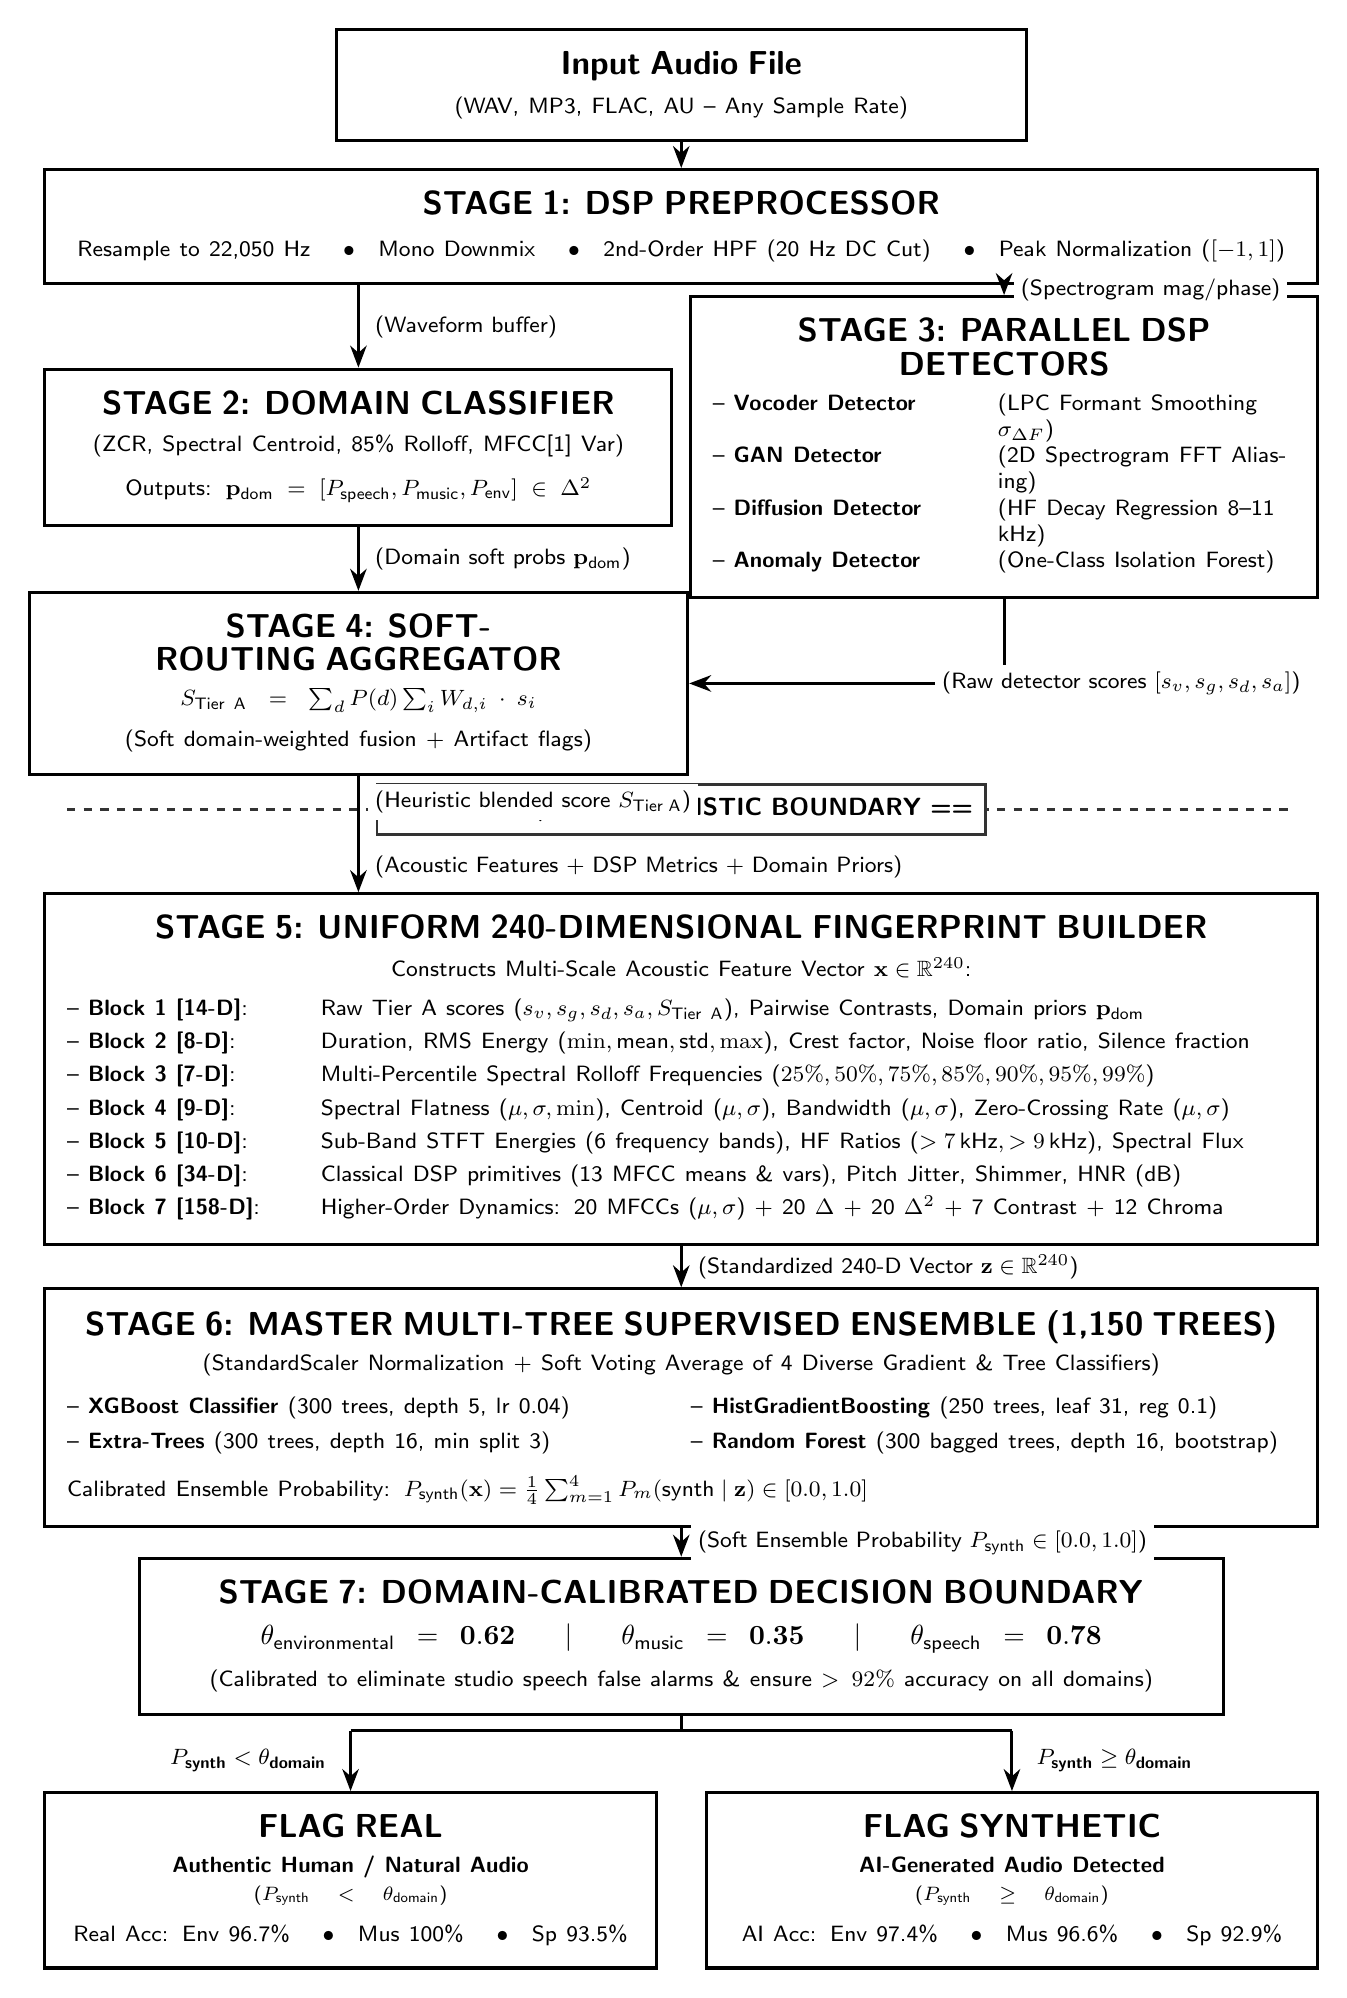
\begin{tikzpicture}[
    >=Stealth,
    font=\sffamily,
    % Sharp, crisp black-outline rectangular boxes matching reference style
    block/.style={
        draw=black,
        rectangle,
        line width=1.1pt,
        fill=white,
        align=center,
        inner sep=8pt
    },
    bulletblock/.style={
        draw=black,
        rectangle,
        line width=1.1pt,
        fill=white,
        align=left,
        inner sep=8pt
    },
    arrowlabel/.style={
        font=\sffamily\footnotesize,
        fill=white,
        inner sep=2.5pt,
        align=center
    },
    flow/.style={
        draw=black,
        line width=1.1pt,
        ->
    }
]

% ==============================================================================
% 1. TOP: INPUT AUDIO FILE (Centered at x=0, y=0)
% ==============================================================================
\node[block, text width=8.2cm] (input) at (0, 0) {
    \textbf{\large Input Audio File}\\[2pt]
    \footnotesize (WAV, MP3, FLAC, AU -- Any Sample Rate)
};

% ==============================================================================
% 2. STAGE 1: DSP PREPROCESSOR (Centered at x=0, y=-1.8)
% ==============================================================================
\node[block, text width=15.6cm] (stage1) at (0, -1.8) {
    \textbf{\large STAGE 1: DSP PREPROCESSOR}\\[3pt]
    \footnotesize Resample to 22,050 Hz \quad$\bullet$\quad Mono Downmix \quad$\bullet$\quad 2nd-Order HPF (20 Hz DC Cut) \quad$\bullet$\quad Peak Normalization ($[-1, 1]$)
};

% ==============================================================================
% 3. STAGES 2 & 3: PARALLEL SENSORY BRANCHES (Strictly Separated: x=-4.1 and x=+4.1)
% ==============================================================================
% Stage 2 (Left): Bounds [-7.8, -0.4], Center at (-4.1, -4.6)
\node[block, text width=7.4cm] (stage2) at (-4.1, -4.6) {
    \textbf{\large STAGE 2: DOMAIN CLASSIFIER}\\[4pt]
    \footnotesize (ZCR, Spectral Centroid, 85\% Rolloff, MFCC[1] Var)\\[4pt]
    \footnotesize Outputs: $\mathbf{p}_{\text{dom}} = [P_{\text{speech}}, P_{\text{music}}, P_{\text{env}}] \in \Delta^2$
};

% Stage 3 (Right): Bounds [+0.4, +7.8], Center at (+4.1, -4.6)
\node[bulletblock, text width=7.4cm] (stage3) at (4.1, -4.6) {
    \centering \textbf{\large STAGE 3: PARALLEL DSP DETECTORS}\\[5pt]
    \footnotesize
    \begin{tabular}{@{}p{3.2cm}p{4.0cm}@{}}
    -- \textbf{Vocoder Detector}   & (LPC Formant Smoothing $\sigma_{\Delta F}$)\\[2pt]
    -- \textbf{GAN Detector}       & (2D Spectrogram FFT Aliasing)\\[2pt]
    -- \textbf{Diffusion Detector} & (HF Decay Regression 8--11 kHz)\\[2pt]
    -- \textbf{Anomaly Detector}   & (One-Class Isolation Forest)
    \end{tabular}
};

% ==============================================================================
% 4. STAGE 4: SOFT-ROUTING AGGREGATOR (Directly under Stage 2 on Left: x=-4.1, y=-7.6)
% ==============================================================================
\node[block, text width=7.8cm] (stage4) at (-4.1, -7.6) {
    \textbf{\large STAGE 4: SOFT-ROUTING AGGREGATOR}\\[3pt]
    \footnotesize $S_{\text{Tier A}} = \sum_d P(d) \sum_i W_{d,i} \cdot s_i$\\[3pt]
    \footnotesize (Soft domain-weighted fusion + Artifact flags)
};

% ==============================================================================
% 5. TIER A / DSP BOUNDARY (y = -9.2)
% ==============================================================================
\draw[black!80, dashed, line width=1.1pt] (-7.8, -9.2) -- (7.8, -9.2);
\node[draw=black!80, fill=white, line width=0.9pt, inner sep=4.5pt, font=\sffamily\small\bfseries] at (0, -9.2) 
    {== TIER A / DSP HEURISTIC BOUNDARY ==};

% ==============================================================================
% 6. STAGE 5: UNIFORM 240-DIMENSIONAL FINGERPRINT BUILDER (Centered at x=0, y=-12.5)
% ==============================================================================
\node[bulletblock, text width=15.6cm] (stage5) at (0, -12.5) {
    \centering \textbf{\large STAGE 5: UNIFORM 240-DIMENSIONAL FINGERPRINT BUILDER}\\[4pt]
    \centering \footnotesize Constructs Multi-Scale Acoustic Feature Vector $\mathbf{x} \in \mathbb{R}^{240}$:\\[6pt]
    \footnotesize
    \begin{tabular}{@{}p{2.8cm}p{12.4cm}@{}}
    -- \textbf{Block 1 [14-D]}: & Raw Tier A scores ($s_v, s_g, s_d, s_a, S_{\text{Tier A}}$), Pairwise Contrasts, Domain priors $\mathbf{p}_{\text{dom}}$\\[2.5pt]
    -- \textbf{Block 2 [8-D]}:  & Duration, RMS Energy ($\min, \text{mean}, \text{std}, \max$), Crest factor, Noise floor ratio, Silence fraction\\[2.5pt]
    -- \textbf{Block 3 [7-D]}:  & Multi-Percentile Spectral Rolloff Frequencies ($25\%, 50\%, 75\%, 85\%, 90\%, 95\%, 99\%$)\\[2.5pt]
    -- \textbf{Block 4 [9-D]}:  & Spectral Flatness ($\mu, \sigma, \min$), Centroid ($\mu, \sigma$), Bandwidth ($\mu, \sigma$), Zero-Crossing Rate ($\mu, \sigma$)\\[2.5pt]
    -- \textbf{Block 5 [10-D]}: & Sub-Band STFT Energies (6 frequency bands), HF Ratios ($>7\,\text{kHz}, >9\,\text{kHz}$), Spectral Flux\\[2.5pt]
    -- \textbf{Block 6 [34-D]}: & Classical DSP primitives (13 MFCC means \& vars), Pitch Jitter, Shimmer, HNR (dB)\\[2.5pt]
    -- \textbf{Block 7 [158-D]}:& Higher-Order Dynamics: 20 MFCCs ($\mu, \sigma$) + 20 $\Delta$ + 20 $\Delta^2$ + 7 Contrast + 12 Chroma
    \end{tabular}
};

% ==============================================================================
% 7. STAGE 6: MASTER MULTI-TREE SUPERVISED ENSEMBLE (Centered at x=0, y=-16.8)
% ==============================================================================
\node[bulletblock, text width=15.6cm] (stage6) at (0, -16.8) {
    \centering \textbf{\large STAGE 6: MASTER MULTI-TREE SUPERVISED ENSEMBLE (1,150 TREES)}\\[3pt]
    \centering \footnotesize (StandardScaler Normalization + Soft Voting Average of 4 Diverse Gradient \& Tree Classifiers)\\[6pt]
    \footnotesize
    \begin{tabular}{@{}p{7.5cm}p{7.7cm}@{}}
    -- \textbf{XGBoost Classifier} (300 trees, depth 5, lr 0.04) & -- \textbf{HistGradientBoosting} (250 trees, leaf 31, reg 0.1)\\[3pt]
    -- \textbf{Extra-Trees} (300 trees, depth 16, min split 3) & -- \textbf{Random Forest} (300 bagged trees, depth 16, bootstrap)
    \end{tabular}\\[6pt]
    \centering \footnotesize Calibrated Ensemble Probability: $P_{\text{synth}}(\mathbf{x}) = \frac{1}{4} \sum_{m=1}^4 P_m(\text{synth} \mid \mathbf{z}) \in [0.0, 1.0]$
};

% ==============================================================================
% 8. STAGE 7: DOMAIN-CALIBRATED DECISION BOUNDARY (Centered at x=0, y=-19.7)
% ==============================================================================
\node[block, text width=13.2cm] (decision) at (0, -19.7) {
    \textbf{\large STAGE 7: DOMAIN-CALIBRATED DECISION BOUNDARY}\\[3pt]
    \normalsize
    $\theta_{\text{environmental}} = \mathbf{0.62} \quad\mid\quad \theta_{\text{music}} = \mathbf{0.35} \quad\mid\quad \theta_{\text{speech}} = \mathbf{0.78}$\\[3pt]
    \footnotesize (Calibrated to eliminate studio speech false alarms \& ensure $>92\%$ accuracy on all domains)
};

% ==============================================================================
% 9. LEAF DECISION OUTPUTS (x=-4.2 and x=+4.2, y=-22.8, Width=7.2cm)
% ==============================================================================
\node[block, text width=7.2cm] (real) at (-4.2, -22.8) {
    \textbf{\large FLAG REAL}\\[3pt]
    \footnotesize \textbf{Authentic Human / Natural Audio}\\[2pt]
    \scriptsize ($P_{\text{synth}} < \theta_{\text{domain}}$)\\[3pt]
    \footnotesize Real Acc: Env 96.7\% \quad$\bullet$\quad Mus 100\% \quad$\bullet$\quad Sp 93.5\%
};

\node[block, text width=7.2cm] (synth) at (4.2, -22.8) {
    \textbf{\large FLAG SYNTHETIC}\\[3pt]
    \footnotesize \textbf{AI-Generated Audio Detected}\\[2pt]
    \scriptsize ($P_{\text{synth}} \ge \theta_{\text{domain}}$)\\[3pt]
    \footnotesize AI Acc: Env 97.4\% \quad$\bullet$\quad Mus 96.6\% \quad$\bullet$\quad Sp 92.9\%
};

% ==============================================================================
% CONNECTING ARROWS & LABELS (Clean, Explicit Node Endpoints)
% ==============================================================================

% Input -> Stage 1
\draw[flow] (input.south) -- (stage1.north);

% Stage 1 -> Stage 2 (Left Branch: downwards from Stage 1 into Stage 2)
\draw[flow] (stage1.south -| stage2.north) -- (stage2.north)
    node[midway, right=3pt, arrowlabel] {(Waveform buffer)};

% Stage 1 -> Stage 3 (Right Branch: downwards from Stage 1 into Stage 3)
\draw[flow] (stage1.south -| stage3.north) -- (stage3.north)
    node[midway, right=3pt, arrowlabel] {(Spectrogram mag/phase)};

% Stage 2 -> Stage 4
\draw[flow] (stage2.south) -- (stage4.north)
    node[midway, right=3pt, arrowlabel] {(Domain soft probs $\mathbf{p}_{\text{dom}}$)};

% Stage 3 -> Stage 4 (Elbow: drops down to y=-7.6 then goes directly into stage4.east)
\draw[flow] (stage3.south) -- (4.1, -7.6) -- (stage4.east)
    node[pos=0.25, right=3pt, arrowlabel] {(Raw detector scores $[s_v, s_g, s_d, s_a]$)};

% Stage 4 -> Stage 5 (Straight vertical drop from stage4.south into stage5.north)
\draw[flow] (stage4.south) -- (stage4.south |- stage5.north)
    node[pos=0.22, right=3pt, arrowlabel] {(Heuristic blended score $S_{\text{Tier A}}$)}
    node[pos=0.78, right=3pt, arrowlabel] {(Acoustic Features + DSP Metrics + Domain Priors)};

% Stage 5 -> Stage 6
\draw[flow] (stage5.south) -- (stage6.north)
    node[midway, right=3pt, arrowlabel] {(Standardized 240-D Vector $\mathbf{z} \in \mathbb{R}^{240}$)};

% Stage 6 -> Decision Boundary
\draw[flow] (stage6.south) -- (decision.north)
    node[midway, right=3pt, arrowlabel] {(Soft Ensemble Probability $P_{\text{synth}} \in [0.0, 1.0]$)};

% ==============================================================================
% Stage 7 Decision Boundary -> Leaves (Connected Tree Fork)
% ==============================================================================
\coordinate (fork_center) at (0, -20.9);
\coordinate (real_fork) at (-4.2, -20.9);
\coordinate (synth_fork) at (4.2, -20.9);

% Vertical stem from Stage 7 bottom to fork level
\draw[line width=1.1pt] (decision.south) -- (fork_center);

% Horizontal crossbar from left fork to right fork
\draw[line width=1.1pt] (real_fork) -- (synth_fork);

% Drop from real_fork into FLAG REAL
\draw[flow] (real_fork) -- (real.north)
    node[midway, left=5pt, font=\sffamily\footnotesize\bfseries] {$P_{\text{synth}} < \theta_{\text{domain}}$};

% Drop from synth_fork into FLAG SYNTHETIC
\draw[flow] (synth_fork) -- (synth.north)
    node[midway, right=5pt, font=\sffamily\footnotesize\bfseries] {$P_{\text{synth}} \ge \theta_{\text{domain}}$};

\end{tikzpicture}
\end{document}
